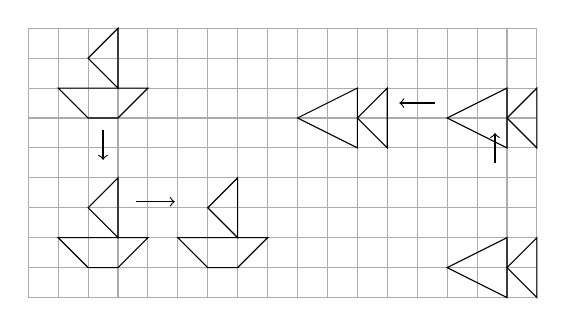
\begin{tikzpicture}[x=.38cm,y=.38cm]\draw[step=1,gray!65] (0,0) grid (17,9);\foreach \x/\y in {0/0,0/5,4/5}{\begin{scope}[shift={(\x,9-\y)},yscale=-1]\draw (1,2)--(2,3)--(3,3)--(4,2)--cycle;\draw (3,0)--(2,1)--(3,2)--cycle;\end{scope}}\foreach \x/\y in {0/0,5/0,5/5}{\begin{scope}[shift={(\x,9-\y)},yscale=-1]\draw (9,3)--(11,2)--(11,4)--cycle;\draw (11,3)--(12,2)--(12,4)--cycle;\end{scope}}\draw[->] (2.5,5.6)--(2.5,4.6);\draw[->] (3.6,3.2)--(4.9,3.2);\draw[->] (15.6,4.5)--(15.6,5.5);\draw[->] (13.6,6.5)--(12.4,6.5);\end{tikzpicture}
